\documentclass[]{article}

\usepackage{pdfpages}

\begin{document}


A qualitative statement of the problem, for context:

\begin{quote}
An arbitrary waveform, given in the frequency domain as $F(\omega)$, propagates through a dispersive, lossy medium. It then drives a damped harmonic oscillator that is initially at rest. \\

What $F$ produces the peak {\it transient} amplitude on the oscillator?

\end{quote}

(this might be completely ill-posed or otherwise intractable - I grasp very little of the below, unfortunately)

(there're lots of different approaches to this - Oughston's asympototic method, Macke and Segard - but this one seems sensible) \\

Zhu et al, in doi: 10.1109/APS.2012.6348428 offer a method to maximize the electric field $e_x(z,t)$, (see Franzen's fourier-transform method \\ http://www.dtic.mil/docs/citations/ADA371944)\\

Prof. Costas gave me a page (unpublished it seems) with more details - see the blue attached pdf.\\

Given

$$ e_x(z,t) = \frac{1}{\sqrt{2 \pi}} \int_{-\infty}^{+\infty}{F(\omega) e^{- j (\omega/c_0)n(\omega)z}\ e^{j\omega t} d\omega} $$

$$W = \frac{1}{\eta_0} \int_{-\infty}^{+\infty}{(n_r(\omega))\ |F(\omega)|^2}\ d\omega$$\\

Where $n(\omega)$ is a complex refractive index per Debye relaxation equation, $n_r()$ is the real part of the same, everything else is a real constant. Set up a functional with a lagrange multiplier\\

$$\xi = -e_x(z,t) + \lambda W$$\\

Take the functional ("variational") gradient with respect to $F(\omega)$.

$$ \nabla \xi = -\frac{1}{\sqrt{2\pi}} \left(e^{- j (\omega/c_0)n(\omega)z}\right)^\star \  e^{-j\omega T} + \lambda...$$

Where * is the complex conjugate.\\

The $\nabla H() = H()^\star$ thing seems to come from Franks, Signal Theory, 1969, page 140 onwards; I cannot make heads or tails of his formulation. \\

Neither Mathematica's VariationalD, Matlab's Fundiff, nor Maple's functionalDerivative seem to yield any meaningful result for grad xi.\\



Then set

$$\nabla \xi = 0$$

and solve for $F(\omega)$ normally. (then fourier transform back to $F(t)$, whatever)


\section{Harmonic oscillator Green's function}

From the below pdf, (renamed F(force) to $e_x$ to avoid confusion), where q is a charge, oscillation amplitude is


$$x(t) = \int_{-\infty}^{+\infty}{G(t,t')\ \frac{q\cdot e_x(z,t'))}{m}\ } dt'$$\\

Where G() is listed therein (eq. 15, for the underdamped case) (Keeping the Green function in the frequency-domain could maybe simplify things a bit? Wouldn't have to fourier-transform back and forth?)\\

Anyhow, then modify the lagrange multiplier,

$$\xi = -x(t) + \lambda W$$\\

And now,

$$\nabla \xi = 0$$

That seems to be the hard part.\\

How do you take the functional derivative of such an equation?


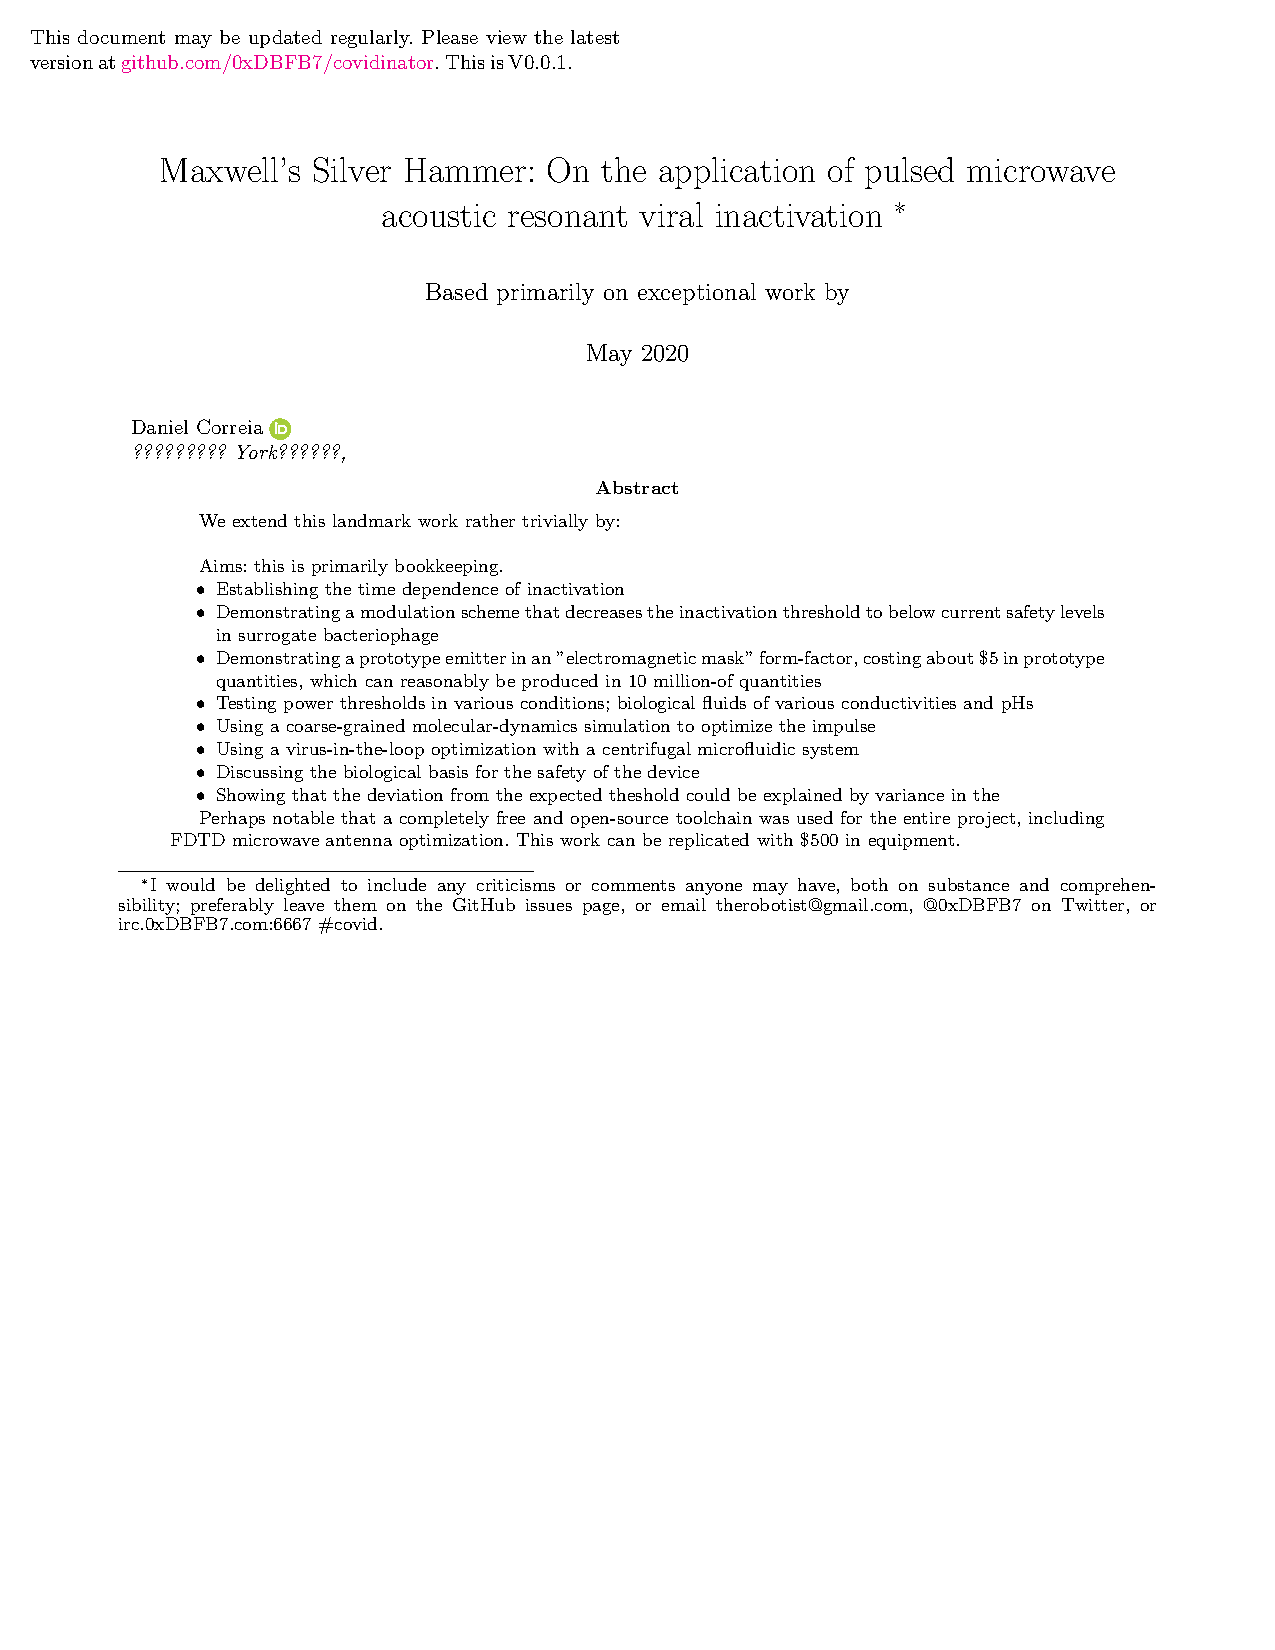
\includepdf[pages=-,pagecommand={}]{paper.pdf}

\includepdf[pages=-,pagecommand={}]{10_greens_function.pdf}


\end{document}
